\documentclass[11pt]{article}  % include bezier curves
\renewcommand\baselinestretch{1.0}           % single space

\oddsidemargin -10 true pt      % Left margin on odd-numbered pages.
\evensidemargin 10 true pt      % Left margin on even-numbered pages.
\marginparwidth 1.5 true in    % Width of marginal notes.
\oddsidemargin  0 true in       % Note that \oddsidemargin=\evensidemargin
\evensidemargin 0 true in
\topmargin -0.5 true in        % Nominal distance from top of page to top of
\textheight 9.0 true in         % Height of text (including footnotes and figures)
\textwidth 6.5 true in        % Width of text line.
\parindent=0pt                  % Do not indent paragraphs
\parskip=0.15 true in
%\usepackage{color}              % Need the color package
\usepackage{hyperref}
\usepackage[pdftex]{color, graphicx}
%\usepackage{graphicx} %for epsfig
\usepackage{graphics}
\usepackage{subfig}
\usepackage{epsfig}
\usepackage{latexsym}
\usepackage{mathrsfs}
\usepackage{eufrak}
\usepackage{amsmath}
\usepackage{graphicx}
\usepackage{longtable}
\usepackage{afterpage}


\title{M3D-C1: Current Status and Future Development in Mode Switch}
\author{Fan Zhang, Seegyoung Seol, Mark S. Shephard} 
\begin{document} 
\maketitle

\tableofcontents
\clearpage
\section{Introduction}
This document overviews the current status of the software that SCOREC provides to M3D-C1 \cite{jardin2004triangular,jardin2007high,ferraro2009calculations,jardin2012review,jardin2012multiple, Ferraro2011, Ferraro2014} and the requirements of the new capability that enables M3D-C1 to switch between  modes. M3D-C1  applies C$^1$  4$^{th}$ order element to solve the magnetohydrodynamics (MHD) equations and simulates the nonlinear instability of the plasma in the tokamak.  The case of non-axis-symmetric instability requires the simulation to be performed on the 3D mesh.  The new  capability  to be developed will allow  M3D-C1  to start with a 2D analysis and switch to 3D when a full 3D discretization is needed.  

The software structure of M3D-C1 is illustrated by Fig. \ref{fig:structure}. The  mesh infrastructure \cite{pumi-web-page,Seol2014} provides the interface to define the geometric model of the tokamak and manages the database of the distributed mesh. The original PDE is discretized over the mesh entities by the Galerkin finite element method \cite{jardin2004triangular,jardin2007high,ferraro2009calculations,jardin2012review,jardin2012multiple}. The element contribution to the stiffness matrix and the force vector \cite{hughes2012finite} is integrated over mesh elements. The mesh infrastructure provides the element connectivity and the geometric information during the discretization of PDE over elements. The global discrete equation is formed from the element-level discrete equation. The DOF ordering is calculated and the global system of the equations is assembled. The parallel communication during the assembly is performed through the localized inter-process communication based on the mesh partition \cite{sahni2009strong,ovcharenko2012neighborhood}.  The global discrete system is solved through the linkage to the equation solvers such as SuperLu \cite{superlu_ug99} and PETSc \cite{petsc-web-page}. There is the procedure that assess the solution quality and improve the mesh if needed through local mesh modification \cite{li20053d,sahni2007automated, lu2013parallel}.

\begin{figure}[hbt]
\center

\includegraphics[width=0.6\textwidth]{fig/m3dc1Structure.png}
\caption{Software structure of M3D-C1} \label{fig:structure}
\end{figure}

The SCOREC group provides the underlying mesh infrastructure, the mesh improvement capability, and the procedures to interact with the mesh infrastructure. The following sections discuses the current capabilities that The SCOREC group provides and the new capability to be developed to support the mode switch in M3D-C1. Section \ref{sec:geo} discusses the tokamak geometry definition in M3D-C1.  Section \ref{sec:mesh} discusses the meshing capabilities of M3D-C1. Section \ref{sec:parallel} discusses the procedures that interact with mesh infrastructure.  Section \ref{sec:futuredevelop} discuses the future development to support the mode switch of M3D-C1. An appendix is provided that describes the function list and verification tools.
\section{Geometry Definition}  \label{sec:geo}
This section describes the geometric components of the tokamak that need to be constructed in M3D-C1. 
The complete geometry is defined by the topological structure and the shape information of the geometric entities. 
\subsection{Geometric Description of the Tokamak}
Tokamak fusion reactors \cite{wesson2011tokamaks} are applied as the experimental approach to study magnetically confined sustainable fusion reactions. The basic tokamak is a torus that is symmetric along
the toroidal direction. The fusion material in a tokamak exists as the state of plasma which is confined by the magnetic field \cite{chen1984introduction}.  M3D-C1 studies the behaviors
of plasma in tokamaks.

Fig. \ref{fig:geo} illustrates the geometric components of the tokamak cross section \cite{wesson2011tokamaks,stacey1982fusion}.  Two coordinate systems,  $(R,Z,\varphi)$ and $(r,\theta, \varphi)$, are  applied in the torkamak geometry. $R$ is the major radius that measures the distance to the axis of the torus. $r$ is the minor radius that measures the distance to the magnetic axis on the cross section. $\varphi$ and $\theta$ are toroidal and poloidal angles respectively. 
The plasma region (9 in Fig. \ref{fig:geo}) is bounded by the limiter or the boundary of the material wall (12 in Fig. \ref{fig:geo}) \cite{wesson2011tokamaks}. There exists a separatrix or the last closed flux surface in plasma (3 in Fig. \ref{fig:geo}) and  it further splits the region into two distinct regions: the plasma core and the scraped-off layer (5 and 4 in Fig. \ref{fig:geo}) \cite{wesson2011tokamaks}. The flux surfaces in the plasma core are concentric loops between the magnetic axis (0 in Fig. \ref{fig:geo}) and the separatrix. The surfaces are distorted away by the x point (6 in Fig. \ref{fig:geo}) which is a saddle point of the magnetic flux on the separatrix.  There can be more than one x points existing on the separatrix in more general situations. The scrape-off layer is the region between the separatrix and the wall boundary. Flux surfaces end at the wall in this region and the outermost surface coincide with the wall.  In addition to the plasma region, the components of the geometry can also include the wall region and an vacuum vessel (8 and 7 in Fig. \ref{fig:geo}).  

\begin{figure}[htb]
\center
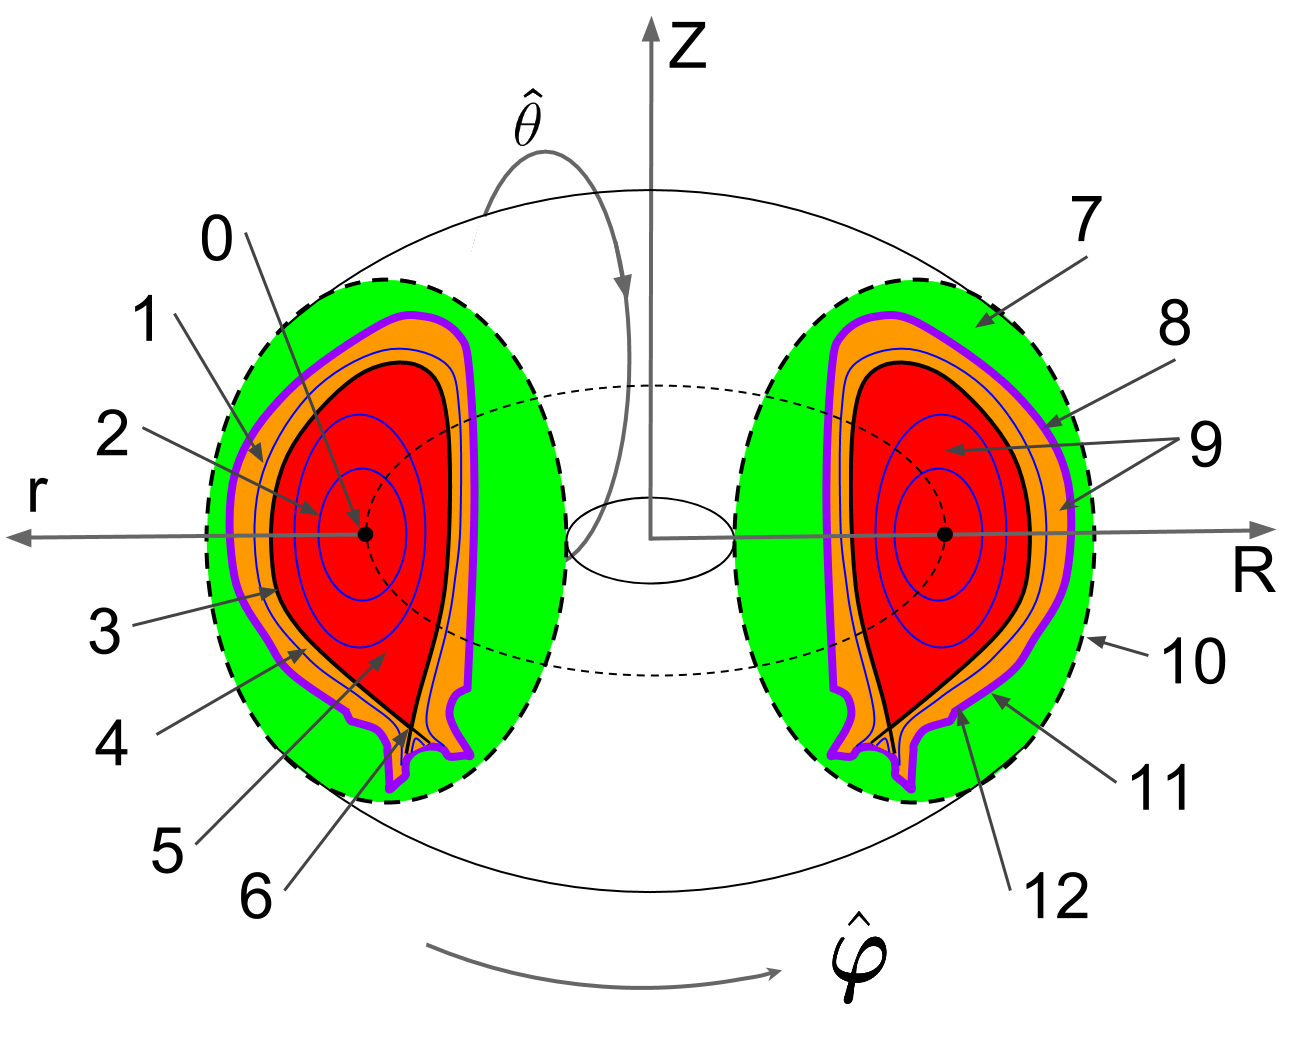
\includegraphics[width=\textwidth]{fig/fusiongeo3d.png}
\caption{Geometric components of the fusion reactor. The coordinate system is $(R,Z, \varphi)$ or $(r,\theta, \varphi)$, where $R$ and $r$ are major and minor radii, and $\varphi$ and $\theta$ are toroidal and poloidal angles. The components include magnetic axis (0), open flux surface (1), closed flux surface (2),  separatrix (3), scrape-off layer (4), plasma core (5), x point (6), vacuum vessel (7), wall region (8),  plasma region (9), vacuum boundary (10), outer wall boundary (11), and inner wall boundary (12).} \label{fig:geo}
\end{figure}

The geometry applied in M3D-C1 is the 3D torus made up by the plasma region, the material wall and the vacuum vessel.  There are planes placed around the torus axis and each plane forms a cross section of the tokamak.
\clearpage
\subsection{Geometry Model Definition in M3D-C1}
The geometric model is defined in terms of the abstraction of the topological entities and their adjacencies \cite{weiler1986topo}. The information that defines the shape of the model entities is associated with the topological entitles. 

The topological entities of the tokamak are regions, that are bounded by shells, which are made up by faces, that are bounded by loops, which are made up of edges, that are bounded by vertices. The topological structure of the geometry entities is summarized below.
\begin{itemize}
\item The 3D torus is made up by regions between the planes (Fig. \ref{fig:3dtopo}). There are up to three regions between two planes that correspond to the  plasma, the wall and vacuum in the tokamak reactor (9, 8 and 7 in Fig. \ref{fig:geo}). 
\begin{figure}[htb]
\center
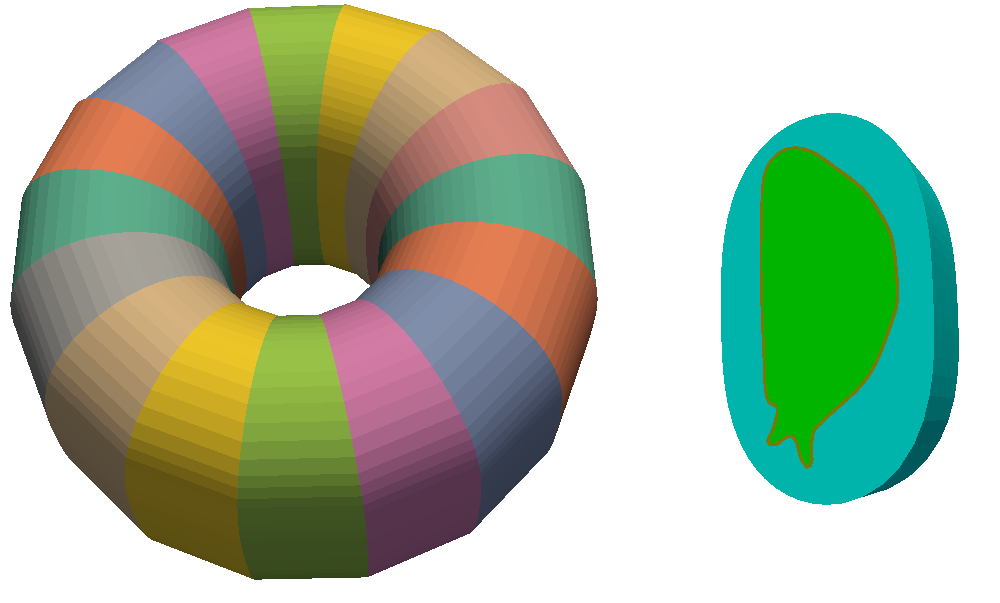
\includegraphics[width=0.8\textwidth]{fig/3dGeoTorus.png}
\caption{The 3D torus with 16 planes. The regions between planes correspond to the plasma, wall and vacuum in Fig. \ref{fig:geo}.} \label{fig:3dtopo}
\end{figure}

\item A region is bounded by a shell that is made up of two faces on the neighboring planes and a number of faces between planes (Fig. \ref{fig:regiontopo}). The faces between planes are on the boundaries of the material wall or the vacuum (12, 11 and 10 in Fig. \ref{fig:geo}). The geometry is non-manifold \cite{weiler1986topo} that each face except that on the vacuum boundary is used to form two regions. 
\begin{figure}[htb]
\center
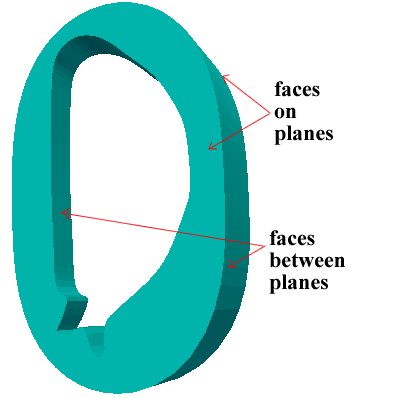
\includegraphics[width=0.4\textwidth]{fig/vacuumGeoRegionFace.png}
\caption{The geometric region of the vacuum between two planes} \label{fig:regiontopo}
\end{figure}

\item There are three faces on a plane (Fig. \ref{fig:facetopo}). The inner  plasma face is bounded by the loop on the inner material wall (loop 1 in Fig. \ref{fig:facetopo}). The wall face is bounded by two loops on the inner and outer material walls (loop 1' and loop 2 in Fig. \ref{fig:facetopo}). The outer vacuum face is bounded by the loop on the outer material wall and the loop on the vacuum vessel (loop 2' and loop 3 in Fig. \ref{fig:facetopo}). The loops that two faces contact on the plane are formed by the same group of edges in the opposite directions. 
\begin{figure}[htb]
\center
\begin{tabular}{ccc}
\subfloat[plasma face]{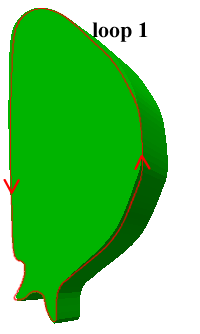
\includegraphics[scale=0.4]{fig/plasmaGeoRegion.png}}
 & \subfloat[wall face]{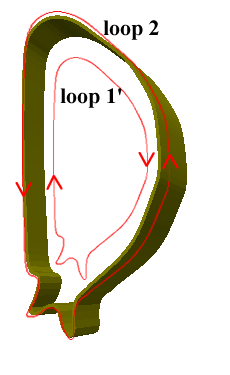
\includegraphics[scale=0.4]{fig/wallGeoRegion.png}}
 & \subfloat[vacuum face]{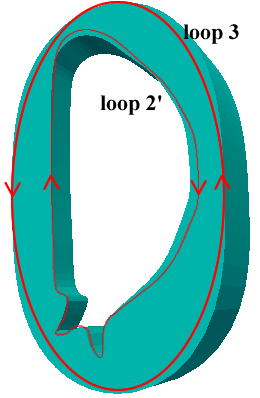
\includegraphics[scale=0.4]{fig/vacuumGeoRegion.png}}
\end{tabular}
\caption{Geometric faces on the plane} \label{fig:facetopo}
\end{figure}

\item The face between planes (Fig. \ref{fig:facetopobtw}) is either bounded by one loop that are made up of two edges on the planes and  two edges between planes, or two loops on the planes.
\end{itemize}
\begin{figure}[htb]
\center
\begin{tabular}{cc}
\subfloat[face bounded by one loop]{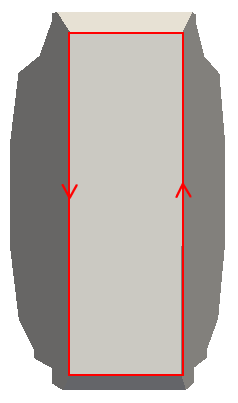
\includegraphics[scale=0.5]{fig/facebtw1.png}}
 & \subfloat[face bounded by two loops]{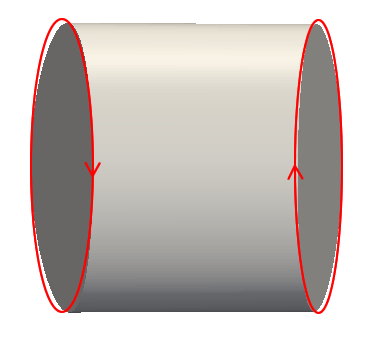
\includegraphics[scale=0.5]{fig/facebtw2.png}}
\end{tabular}
\caption{Geometric faces between planes} \label{fig:facetopobtw}
\end{figure}

In addition to the topological structure, the shape information defines the complete geometry model of the tokamak  geometry. The shape information are the positions of the model vertices, the geometry of the curves associated with the model edges, and the geometry of the surfaces associated with the model faces.  Ideally the geometry of the wall curves would be that defined in the reactor's CAD model. Currently the wall curves is defined by an ordered set of points and the points are interpolated by the B-splines \cite{prautzsch2002bezier}. They can also be defined by user-specified analytic functions. The curve of the vacuum boundary is defined as a simple smooth loop formed by B-spline given the user-specified width and height. The surfaces are either planar or formed by revolving the curves along the torus axis.

\afterpage{\clearpage}
\section{Meshing Capabilities} \label{sec:mesh}
This section discuses the meshing capacities of M3D-C1.  Meshes on each cross section (plane) are identical. The 3D mesh is constructed by forming wedge elements between the planes.  

The relation between the mesh and the geometry is maintained during the meshing procedure. Each mesh entity is classified on a specific geometric entity \cite{shephard2000meshing,beall2004comparison,pumi-homepage}. The mesh-geometry classification gives the necessary information to generate the unstructured mesh that is consistent to the geometry. It determines the validity of mesh operations and provides geometric information during the mesh modification. The information of mesh-geometry classification also determines the set of the governing equation applied in a specific type of the region (plasma, wall or vacuum).

\subsection{Mesh Generation and Improvement on Tokamak Cross Section}
The initial mesh on a cross section of the tokamak is generated by the Simmetrix meshing tool \cite{simmetrix-web-page}. If the face is bounded by a simple loop (Fig. \ref{fig:facetopobtw}.b), a coarse mesh with several elements can be generated manually and the initial mesh is obtained by uniformly refining the coarse mesh. 

The initial mesh is further improved by applying the local modification iteratively until the mesh meets the desired size field \cite{li2003accounting,li20053d,alauzet2006parallel,sahni2007automated}. Currently, a mesh size field is defined from the toroidal magnetic flux field $\psi$. A normalized flux field is defined by $\tilde{\psi}=\frac{\psi-\psi_0}{\psi_l-\psi_0}$, where $\psi_l$ and $\psi_0$ is the field value at the plasma boundary and the magnetic axis. The mesh size normal to the surface $h_1$ and the mesh size tangent to the surface $h_2$ is defined as

\begin{equation}
h_i^{-1}=\tilde{h}_i^{-1}+\frac{1}{l_{ci}\left(1+\frac{\tilde{\psi}-\psi_c}{W_c}\right)^2}, \quad i=1,2
\end{equation}

where $l_{ci}$, $\psi_c$ and $W_c$ are constants. 
$\tilde{h}_i$ is defined by
\begin{eqnarray}
\tilde{h}_i&=&b_i[1-e^{|\frac{\tilde{\psi}}{a}-1|^2)}]+c_i, \quad \tilde{\psi}<a,\, \text{inside plasma} \nonumber \\ 
\tilde{h}_i&=&d_i[1-e^{|\frac{\tilde{\psi}}{a}-1|^2)}]+c_i, \quad \tilde{\psi}>a, \, \text{outside plasma}
\end{eqnarray}
where $b_i$, $d_i$, $a$ and $c_i$ are constants. The constant parameters of the equations are determined such the adapted mesh has finer size at the plasma boundary and the region that the instability may happen. Since there is richer physics in the normal direction of the flux surface than the other direction, the directional mesh size field are defined to represent this property.
\subsection{3D Mesh Construction}
The 3D Mesh is constructed by forming wedge elements between the same 2D meshes on the planes. The processes are divided into $N$ groups, where $N$ equals to the number of the planes. Each group of the processes loads the same 2D mesh. Wedge elements are created by connecting the two triangle elements on the neighboring planes.  Fig. \ref{fig:3dmesh} and \ref{fig:3dmeshSlice} illustrates the process.

\begin{figure}[htb]
\center
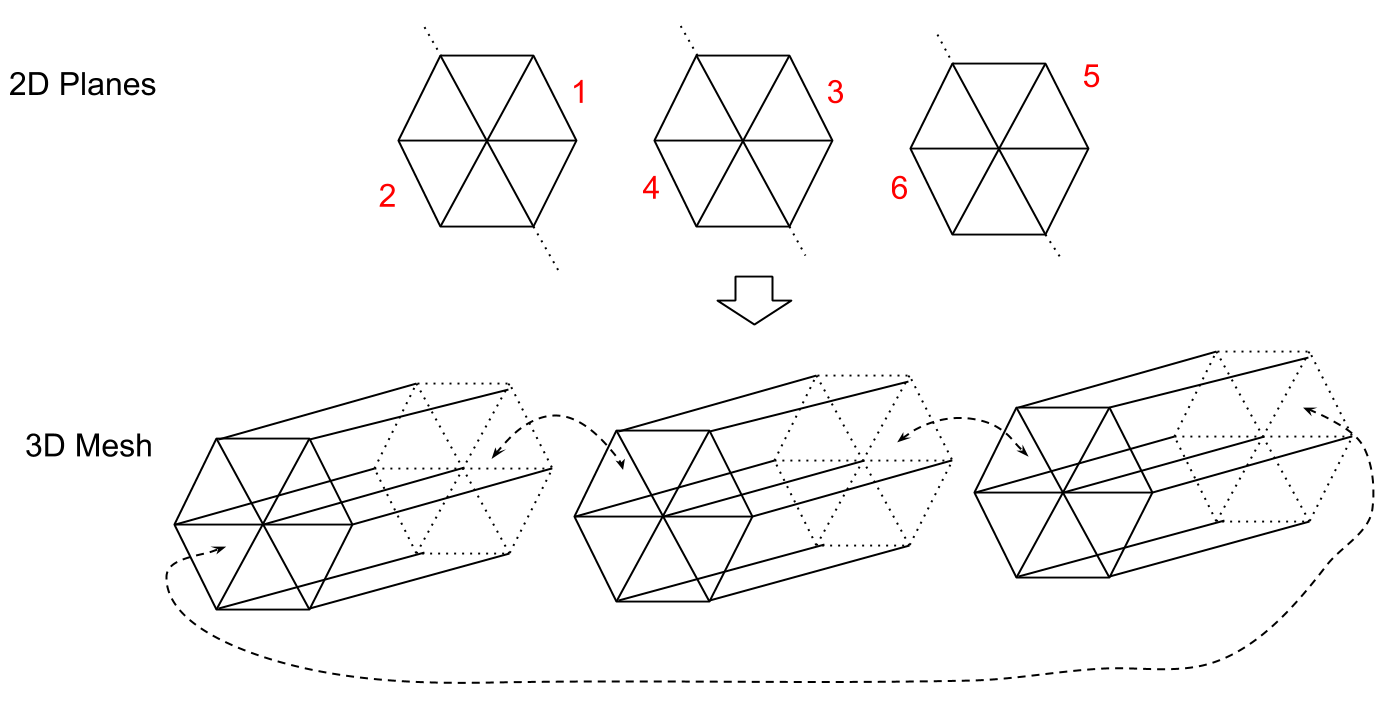
\includegraphics[width=0.8\textwidth]{fig/3dmesh.png}
\caption{The process of constructing 3D mesh. There are 6 processes and 3 planes. The dotted elements are remote copies at the mesh-part boundary (see \cite{pumi-web-page}).} \label{fig:3dmesh}
\end{figure}

\begin{figure}[htb]
\center
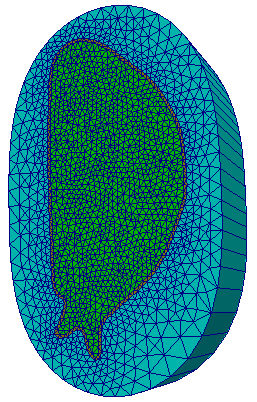
\includegraphics[width=0.5\textwidth]{fig/3dmeshSlice.png}
\caption{Wedge elements between planes} \label{fig:3dmeshSlice}
\end{figure}
\afterpage{\clearpage}
\section{Procedures to Interact with  Mesh Infrastructure} \label{sec:parallel}
This section discusses the procedures that interact between the underlying mesh infrastructure and the physics analysis code in M3D-C1 (Fig. \ref{fig:structure}).  The mesh infrastructure provides the information of the distributed mesh and the geometry that the mesh is classified on. Procedures that link  physics analysis code of M3D-C1 to the underlying mesh infrastructures  are developed. The procedures take the information from the mesh infrastructure and  compute the necessary inputs for use by the physics analysis. The procedure of mesh improvement through local modification also relies on the mesh infrastructure. The following paragraphs discuss the procedures that control the information flow between the mesh infrastructure and each specific component in M3D-C1.

The process of the PDE discretization over elements needs the information of the mesh entities and the geometric entities that the mesh entities are classified on. The procedure that inquires  the underlying mesh database and passes the information to the PDE discretization process is provided.  The mesh-entity-level information includes the connectivity of the element and the node position. The mesh-geometry classification identifies the set of the governing equation applied in a specific type of the region. The geometric shape such as the normal direction and curvature provides the necessary boundary information during the  PDE discretization process \cite{jardin2010computational}.

The process to form the global discrete equation needs the global DOF ordering and the procedure to assemble the global system of the equations. The global DOF ordering assigns a unique integer to the DOF's associated with mesh entities based on the mesh-adjacency information that improves the data locality \cite{zhou2010adjacency}. The parallel communication to assemble the global system of the equations is performed through the localized inter-process communication based on the mesh partition \cite{sahni2009strong,ovcharenko2012neighborhood}.  The connection and ownership between remote copies of mesh vertices \cite{Seol2014} at the part boundary is obtained form the mesh infrastructure and the elemental contribution to the stiffness matrix and the force vector is assembled by passing information between remote copies. Fig. \ref{fig:msgpassformat}.a illustrates the process. The non-owned vertices (hallowed circles) send the  the elemental contribution to the stiffness matrix and the force vector to owned vertices (solid circles) and the complete values are assembled.

\begin{figure}[htb]
\center
\begin{tabular}{cc}
%\subfloat[assemble]{\includegraphics[height=4cm]{fig/messagePassing2D.png}}
% & \subfloat[synchronize]{\includegraphics[height=4cm]{fig/messagePassing2DSyc.png}}
\end{tabular}
\caption{Inter-process communication between remote copies of mesh vertices. The mesh is partitioned into three parts and loaded by three processes. The dotted lines are boundaries of the mesh parts. The hollowed circles and dashed lines are non-owned mesh entities. The solid circles and lines are owned mesh entities. The arrows show the communication direction.} \label{fig:msgpassformat}
\end{figure}


There are procedures that set up the exterior  parallel equation solvers such as SuperLu \cite{superlu_ug99} and PETSc \cite{petsc-web-page} and return the solution vector to the analysis procedure. The owner vertices send the DOF's of the solution field to the non-owned vertices at the part boundary such that the solution field is synchronized. Fig. \ref{fig:msgpassformat}.b illustrates the process.

The assessment of the solution quality and mesh improvement needs interaction between the solution fields, mesh improvement procedure and the mesh infrastructure.  The correction indicator is calculated from the solution field and it is used to obtain the mesh size field that defines the optimal mesh desired.  The mesh is improved through local modifications \cite{li20053d,sahni2007automated, lu2013parallel} that interacts directly with the mesh infrastructure. Since the mesh is symmetric in the toroidal direction of the tokamak,  it is improved by adapting the 2D mesh on the cross section of the tokamak. The basic types of modifications on the 2D mesh include split, collapse, swap, node repositioning and snap. The mesh element can be refined by the split operation. The collapse operation can be used to coarsen the mesh. Element shapes can be improved by the operation of edge swap and node repositioning. Nodes classified on the geometric boundary are moved to the snapped position during mesh adaptation such that the consistency to the original geometry is maintained. These basic types of mesh modifications are further combined as the compound operations which provide more flexible ways to mesh improvement.

Solution fields on the original mesh can be easily transferred to the new mesh with the controlled error during the local mesh modification.  The process of solution transfer is to determine the DOF's of the field on the new mesh. The DOF's are attached to mesh vertices in M3D-C1 \cite{jardin2004triangular,jardin2012multiple} and correspond to the field value and its derivatives. New DOF's only need to be calculated when a new vertex is created during the operation of edge split or when a mesh vertex is moved during the operations of node repositioning and snap.  The field value and its derivatives on the original mesh are interpolated at the position of the new vertex or the position that the original vertex is moved to. The values of the new DOF's are obtained from the interpolated field value and its derivatives.

\section{Future Development in Mode Switch} \label{sec:futuredevelop}
\subsection{Mode Switch in M3D-C1} \label{sec:modeswitch}
 M3D-C1 studies the non-linear instability of plasma in the tokamak.  If the nonlinear instability is axis-symmetric, the equations are solved on a 2D mesh. In the situation of non-axis-symmetric instability, it needs to solve the equations on a 3D mesh. Currently, M3D-C1 runs in the following three modes.
\begin{itemize}
\item 2D with real numbers (\textit{2D Real})
\item 2D with complex numbers (\textit{2D Complex})
\item 3D with real numbers (\textit{3D Real})
\end{itemize}

In order to support the switch from \textit{2D Real} to \textit{3D Real},
M3D-C1 performs the \textit{2D Real}  simulation, and switch to the \textit{2D Complex} simulation periodically to check whether the non-axis-symmetric instability can happen. And then M3D-C1 switches from \textit{2D Real} to \textit{3D Real}.  The mesh changes from 2D to 3D and the solution of the field migrates from 2D mesh to 3D mesh. 

\subsection{Field In M3D-C1} \label{sec:field}
This section introduces the shape functions associated with the mesh element and the field interpolated by the shape functions in M3D-C1.

The 3D shape functions are defined by taking tensor product of the $C^1$ reduced quintic shape functions and the Hermite cubic polynomials \cite{jardin2004triangular,jardin2012review}.  The DOF's are listed in Table \ref{tab:dofs}.  The coordinate system is $(R,Z,\varphi)$ (Fig. \ref{fig:geo}).  DOF's of the $C^1$ triangle element  correspond to the function value, the first and second derivatives in the $R$ and $Z$ directions.  DOF's of the Hermite cubic polynomials correspond to the function value and the first derivative in the $\varphi$ direction.
\begin{table}
\begin{center}
 \begin{tabular}{|l|l|l|l|l|l|l|}
\hline
group 1 &$d$ & $d_{,R}$ & $d_{,Z}$ & $d_{,RR}$ & $d_{,RZ}$ &$d_{,ZZ}$  \\ \hline
group 2 &$d_{,\varphi}$ & $d_{,R\varphi}$ & $d_{,Z\varphi}$ & $d_{,RR\varphi}$ & $d_{,RZ\varphi}$ &$d_{,ZZ\varphi}$  \\ \hline
\end{tabular}
\caption{DOF's associated with the mesh vertex in M3D-C1} \label{tab:dofs}
\end{center}
\end{table}
A scaler field on the mesh with $N$ vertices is defined as
\begin{equation}
\sum_{i=1}^{NDOF} d_i \mu_i,
\end{equation}
where $d_i$ is the  $i^{th}$ DOF and  $\mu_i$ is the associated shape function. The number of DOF's, $NDOF$, is equal to $6N$ in the 2D mode that only the first group of DOF's in Table \ref{tab:dofs} are used, or is equal to $12N$ in the 3D mode. $d_i$ can either be a complex or real number.

The physics vector fields such as the velocity and the magnetic field are decomposed into scalar fields. For example, the velocity is decomposed into three scalar fields $(U, \omega, \chi)$ \cite{jardin2012multiple} is represented in the cylindrical coordinate $(R,Z, \varphi)$ as
\begin{equation}
\mathbf{V}=R^2\nabla U \times \nabla \varphi + R^2\omega\nabla\varphi+\frac{1}{R^2}\nabla_\perp\chi. \label{3scalars}
\end{equation}
In reduced models, the velocity is decomposed into less scalar fields in the form
\begin{equation}
\mathbf{V}=R^2\nabla U \times \nabla \varphi + R^2\omega\nabla\varphi 
\end{equation}
for the two scalar representation and
\begin{equation}
\mathbf{V}=R^2\nabla U \times \nabla \varphi.
\end{equation}
for the one scalar representation.

Currently, M3D-C1 can export and import the field data through the Adaptable IO System (ADIOS) (\url{https://www.olcf.ornl.gov/center-projects/adios/}). It allows M3D-C1 to check out the field data at some point (for example, running time hits the limit, system maintenance), and check in the data and continue the simulation later. It is a useful capability especially on the massively distributed computing systems that the chance of system failure increases. The √ of exporting and importing the field needs to happen within the same mode (see Sec. \ref{sec:modeswitch} for different modes in M3D-C1). 
\subsection{Future Development}
The future development lies in the following  aspects. 
\begin{enumerate}
\item mode control in M3D-C1. The mode in the physics code (M3D-C1) is controlled by passing different flags during the complication. If the mode needs to be switched during running time, the M3D-C1 needs to be reconstructed.

The SCOREC libraries control the mode by parameters in the functions and the mode can be changed during running time. 
\item a complete mesh representation of 3D mesh. The classification to the partition model needs to be properly maintained. A set of API functions in PUMI that supports modifying partition model during running time is under consideration. \footnote{The old way to change the partition model relies on the specific implementation of the partition model inside PUMI. It was abandoned as PUMI evolves. } 
\item field migration between the different modes through files or memories. The second type of switch needs to address the issue to map simulation results from 2D mesh to the 3D mesh.

 A high-level description of new functions needed  are listed as follows.
  
\begin{itemize}
\item
\begin{verbatim}
obtain_field( <in> vertexIdentifier,
             <in> planeIdentifier,
             <in> data_source,
             <out> buffer )
\end{verbatim}
Given the mesh vertex identifier and the plane identifier, obtain the field associated with the vertex and fill the data into the buffer. The data may come from memory (previous simulation results) or from file. For the first type switch,  the plane identifier is not needed since both modes are 2D (only one plane). 
\item
\begin{verbatim}
process_field ( <in> vertexIdentifier,
               <in> planeIdentifier,
               <inout> buffer )
\end{verbatim}
 Given the mesh vertex identifier and the plane identifier, process the associated field. In particular, the process adds perturbation to the field.
 \item
\begin{verbatim}  
feed_field ( <in> vertexIdentifier,
            <in> planeIdentifier,
            <in> buffer,
            <out>data_destination)
\end{verbatim}
The procedure feeds back the field associated with mesh vertex to the data destination. The data destination can be  memory if it is a restart of simulation, or file if it is a check point.
\end{itemize}
\end{enumerate}
\subsection{Options to Fulfill the New Capability During Running Time}
This sub section discusses the possible options to fulfill the new capability that migrates the field from 2D mesh to 3D mesh during running time.

The mesh and mesh partition is kept consistent in the 2D and 3D mesh during the mode switch. That is, the mesh on each plane in 3D mesh is the same as that in the 2D mesh.  The purpose is to avoid a global search of field data. Two options are described below.
\begin{itemize}
\item[1] The first option allows some processes to idle at some point (Fig. \ref{fig:wedgePlane}).  Allocate the processes that are need for the simulation on the 3D mesh. Assume there are $M$ planes, and each plane needs $N$ processes. The total number of processes allocated is $MN$. The processes are divided into $M$ groups.

The first group loads the 2D mesh and performs the 2D simulation. The rest groups of processes are just idling till the 3D simulation begins.

All the groups of processes obtain the mesh and field data from the first group that has been doing the 2D simulation. The 3D mesh is constructed by creating wedge elements between planes.  The 2D field data is processed by a pre-defined routine and then assigned to the 3D mesh. 
\begin{figure}[htb]
\center
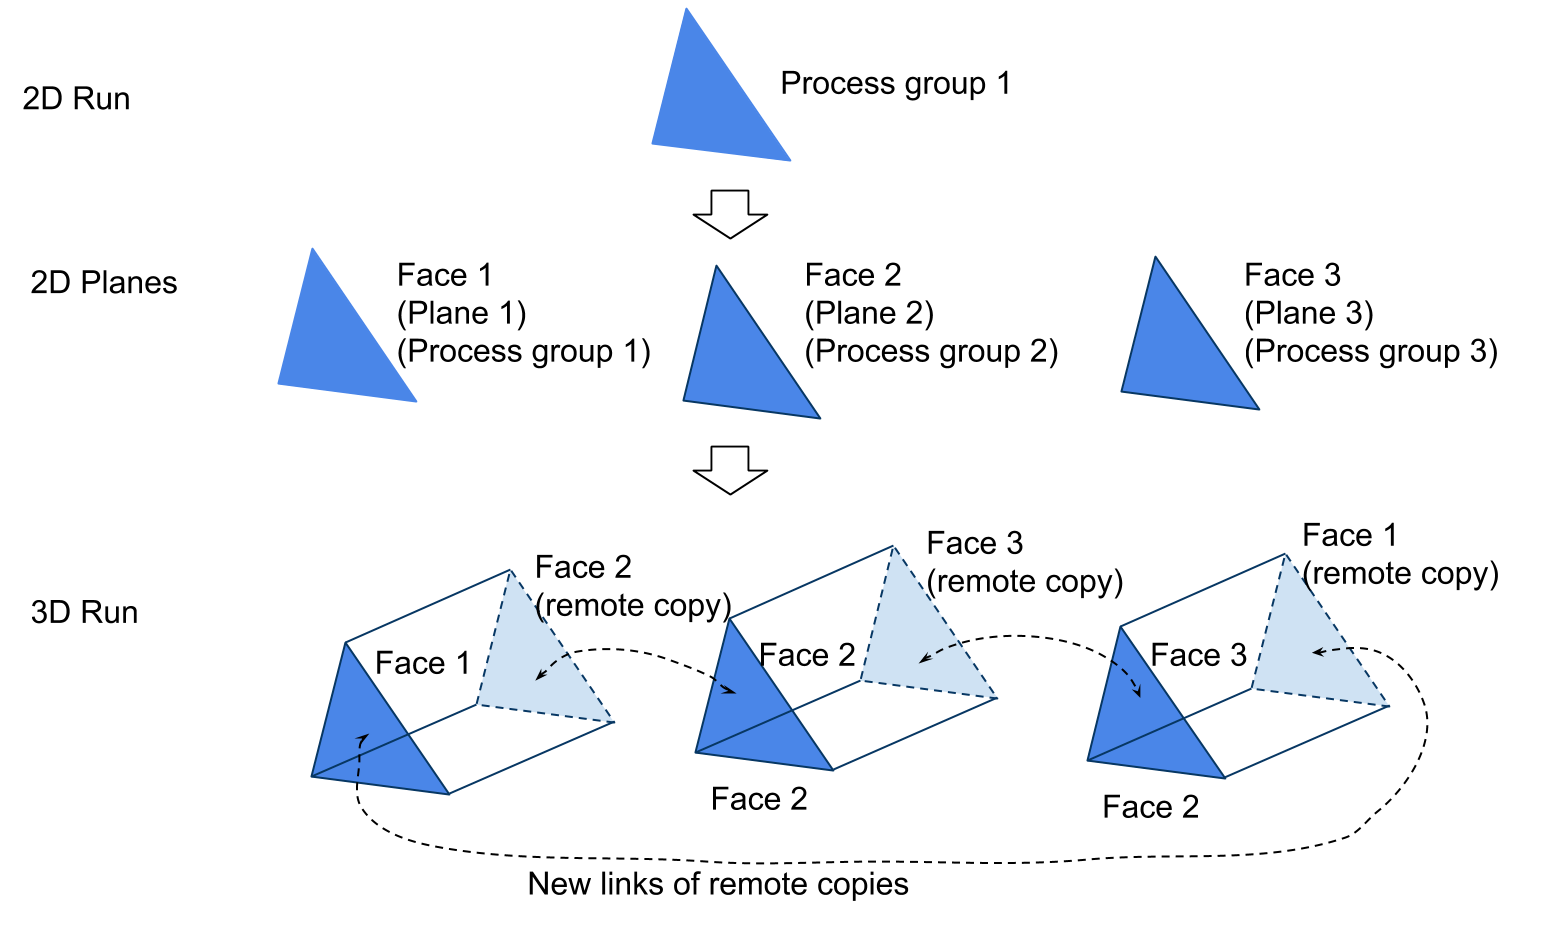
\includegraphics[width=0.8\textwidth]{fig/wedgePlane.png}
\caption{Option 1: idling processes. There are processes idling at the stage of 2D simulation.} \label{fig:wedgePlane}
\end{figure}
\item[2] The second option is to perform 2D simulation with all the processes (Fig. \ref{fig:wedgePlane2}).  Each process loads one part for 2D simulation.

In order to start 3D simulation,  the mesh part is migrated and each process holds multiple parts. For example, initially there are 6 processes that run on the 2D mesh and there are 6 parts of mesh. In order to start a 3D simulation with 3 planes, the mesh part is migrated and redistributed such that each process holds 3 parts of the mesh. Process 1 holds part 1, 2 and 3. Process 2 holds part 3, 4 and 5. Process 3 holds part 1,2,3. Process 3 holds part 4,5 and 6. And so on.

The field migrates with the mesh part.  The  3D mesh is constructed and the 2D field data is processed and assigned to the 3D mesh. 

\begin{figure}[htb]
\center
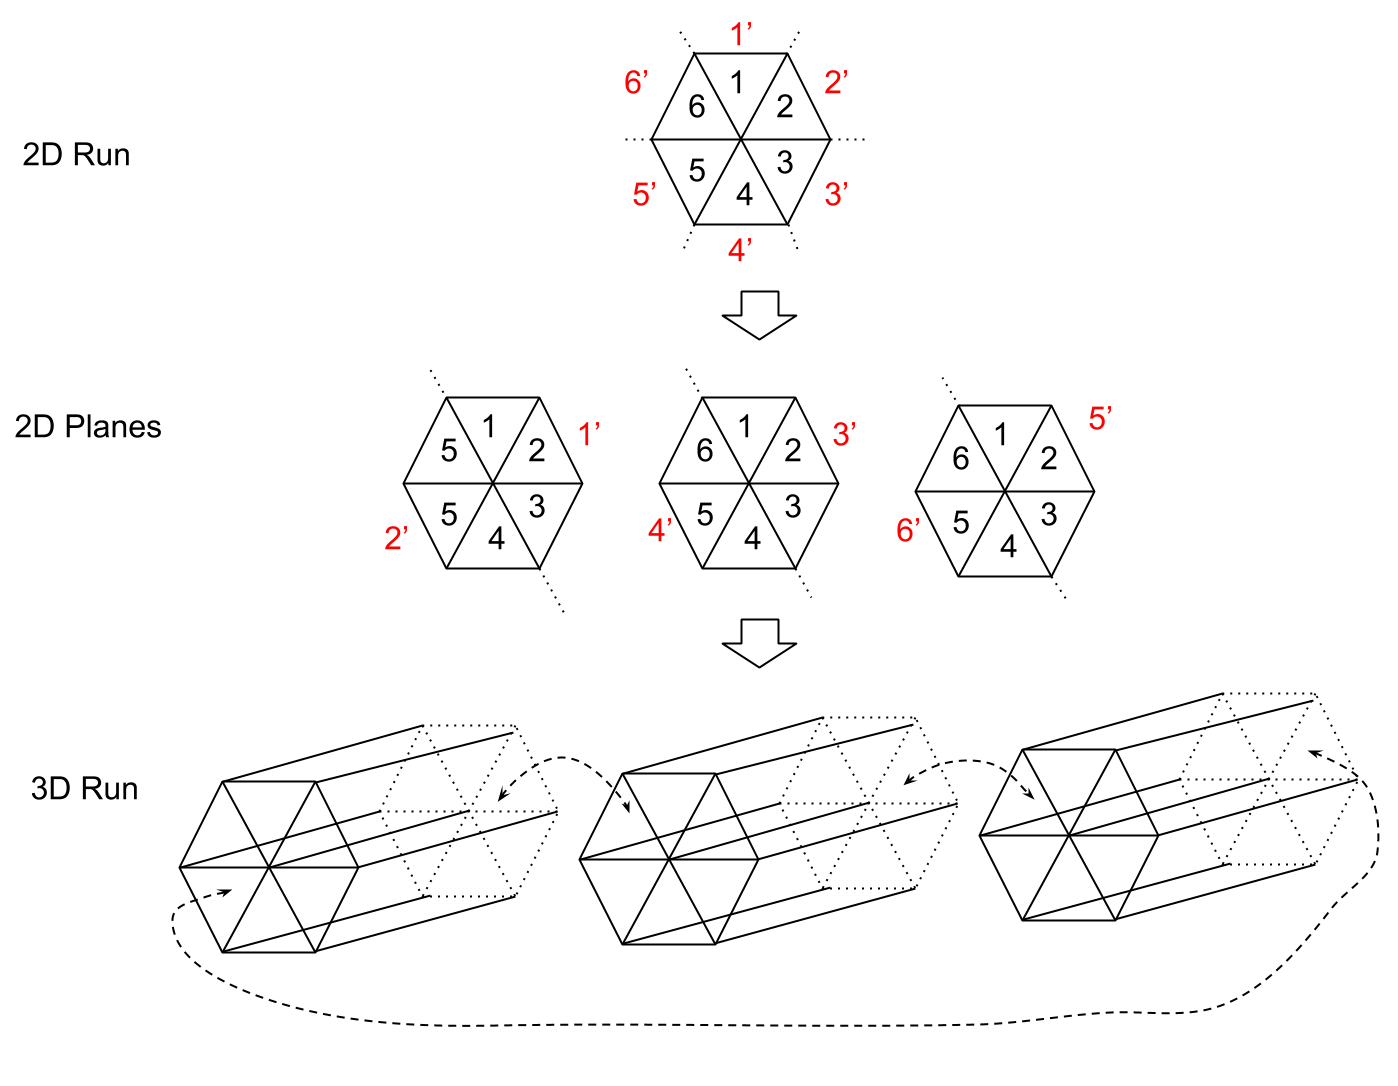
\includegraphics[width=0.8\textwidth]{fig/wedgePlane2.png}
\caption{Option 2: multiple parts on a single process. Each process holds 3 parts on the 3D mesh.} \label{fig:wedgePlane2}
\end{figure}
\end{itemize}

\clearpage
\bibliographystyle{ieeetr}
\bibliography{reference}
\clearpage
\appendix
\section{Software Components}
The following software components from SCOREC are used in M3D-C1.
\begin{itemize}
\item  Parallel Unstructured Mesh Management Infrastructure (PUMI) \cite{pumi-web-page}
\item \emph{MeshAdapt} that  provides services to support mesh topology modification
\end{itemize}

%Efforts to clean up codes are being performed.
%\begin{itemize}
%\item Removing unnecessary files/functions
%\item Replacing obsolete functions with PUMI functions. For instancen $PList$ and $FMDB$. 
%\item Eliminating global and unnecessarily duplicated variables
%\end{itemize}  
%%%%%%%%%%%%%%%%%%%%%%%%%%%%%%%
\section{API Functions}
%%%%%%%%%%%%%%%%%%%%%%%%%%%%%%%
The section describes the specification of API functions provided to the M3D-C1 Fortran driver. The function prototypes are declared in the file \texttt{m3dc1$\_$scorec.h}. Throughout this section, unless specified, mesh entities and DOF's are specified by a local ID. A word ``\emph{global}'' in a function name indicates that the function involves global operation or global data.

%%%%%%%%%%%%%%%%%%%%%%%%%%%%%%%
\subsection{Initialization and finalization}
%%%%%%%%%%%%%%%%%%%%%%%%%%%%%%%
The functions initialize/finalize the PUMI operations.

\begin{verbatim}
// fortran name: m3dc1_domain_init
int m3dc1_scorec_init();
\end{verbatim}\vspace{-.5cm}\hspace{1cm}
Initialize the PUMI service for distributed model and mesh infrastructure. Note that MPI should be initialized prior to this function.

\begin{verbatim}
// fortran name: m3dc1_domain_finalize
int m3dc1_scorec_finalize();
\end{verbatim}\vspace{-.5cm}\hspace{1cm}
Finalize the PUMI service and clears all PUMI related data. Note that MPI finalization should follow.

%%%%%%%%%%%%%%%%%%%%%%%%%%%%%%%
\subsection{Plane}
%%%%%%%%%%%%%%%%%%%%%%%%%%%%%%%

\begin{verbatim}
int m3dc1_plane_setphi(
    int*  /* in */  planeid, 
    double*   /* in */  phi);
\end{verbatim}\vspace{-.5cm}\hspace{1cm}
Given a plane ID and a double, set the phi value of the plane.

\begin{verbatim}
int m3dc1_plane_getphi(
    int*  /* in */  planeid, 
    double*  /* out */  phi);
\end{verbatim}\vspace{-.5cm}\hspace{1cm}
Given a plane ID, return the value of phi of the plane.

%%%%%%%%%%%%%%%%%%%%%%%%%%%%%%%
\subsection{Geometric model}
%%%%%%%%%%%%%%%%%%%%%%%%%%%%%%%

\begin{verbatim}
int m3dc1_model_load (char*  /* in */  model_file);
\end{verbatim}\vspace{-.5cm}\hspace{1cm}
Load a geometric model from a model file that describes the geometry of the 2D cross section of the Tokamak. The file can contain
\begin{itemize}
\item parameters of the user specified analytic expression that defines a single loop as $R(t)=a_1 + a_2cos\left(t + a_3sin(t)\right)$ and $Z(t)= a_4 + a_5sin(t)$.
\item lists of geometric vertex and edges on the wall and vacuum boundaries and parameters of B-splines that define the shape of each edge.
\end{itemize}

\begin{verbatim}
int m3dc1_model_setnumplane (int*  /* in */  num_plane);
\end{verbatim}\vspace{-.5cm}\hspace{1cm}
Given an integer \textit{num$\_$plane}, set the number of planes in 3D. For 2D, the number of plane is 1.

\begin{verbatim}
int m3dc1_model_getnumplane (int*  /* out */  num_plane);
\end{verbatim}\vspace{-.5cm}\hspace{1cm}
Return the number of planes. For 2D, the number of plane is 1.

\begin{verbatim}
int m3dc1_model_getplaneid (int*  /* out */  plane_id);
\end{verbatim}\vspace{-.5cm}\hspace{1cm}
Return the plane ID where the local process belongs. The plane ID starts from 0.

\begin{verbatim}
int m3dc1_model_getedge (
    int*  /* out */  left_edge, 
    int*  /* out */  right_edge,
    int*  /* out */  bottom_edge, 
    int*  /* out */  top_edge); 
\end{verbatim}\vspace{-.5cm}\hspace{1cm}
Return the four model edges of the rectangular domain.

\begin{verbatim}
int m3dc1_model_getmincoord (
    double*  /* out */  x_min, 
    double*  /* out */  y_min);
\end{verbatim}\vspace{-.5cm}\hspace{1cm}
Return the minimum coordinate of the 2D cross section.
	      \textit{x\_min} is the minimum horizontal coordinate value. 
	      \textit{z\_min} is the minimum vertical coordinate value.

\begin{verbatim}
int m3dc1_model_getmaxcoord (
    double*  /* out */  x_max, 
    double*  /* out */  y_max);
\end{verbatim}\vspace{-.5cm}\hspace{1cm}
Return the maximum coordinate of the 2D  cross section. 
          \textit{x\_max} is the maximum horizontal coordinate value. 
          \textit{Y\_max} is the maximum vertical coordinate value.

\begin{verbatim}
int m3dc1_model_print();
\end{verbatim}\vspace{-.5cm}\hspace{1cm}
Display the model information.

%%%%%%%%%%%%%%%%%%%%%%%%%%%%%%%
\subsection{Mesh}
%%%%%%%%%%%%%%%%%%%%%%%%%%%%%%%
When a mesh is distributed in parallel, a mesh entity can be uniquely identified in two ways: (i) an entity dimension and a global entity ID, or (ii) an entity dimension, a process rank and a local entity ID. The entity dimension is 0 for vertex, 1 for edge, 2 for face and 3 for region. For M3D-$C^1$, each mesh vertex has a $node$ serving as DOF holder. A mesh entity of highest dimension (face in 2D and region in 3D) is termed $element$. 

For a distributed mesh on multiple parts, mesh entities not on part boundaries are termed \textit{internal entity} and duplicated mesh entities along part boundaries are termed \textit{part boundary entity}. Among multiple copies of a part boundary entity, one entity is designated to be an \textit{owner copy} and is in charge of updating the rest of copies. The rest of entity copies are termed \textit{non-owned part boundary entity}. For a part boundary entity, duplicate \textit{off-part} copies are termed \textit{remote copy}. All internal entities are owner copies.

To avoid communications between the parts, it is beneficial to support the ability to have a copy of $non$-part boundary entities on other part, referred as $ghosting$. A \textit{ghost copy} is a read-only, duplicated, off-part internal entity copy including global ID, tag data, and field data. Similar to the ownership of part boundary entities, the original owner copy is designated as \emph{owner} of all \textit{ghost copies}.

\begin{verbatim}
int m3dc1_mesh_load (char*  /* in */  mesh_file);
\end{verbatim}\vspace{-.5cm}\hspace{1cm}
Load a mesh from mesh file(s).

\begin{verbatim}
int m3dc1_mesh_build3d ();
\end{verbatim}\vspace{-.5cm}\hspace{1cm}
Construct 3D mesh from multiple 2D planes where each plane is loaded with 2D mesh. 

\begin{verbatim}
// fortran name: m3dc1_ghost_load
int m3dc1_ghost_create (int*  /* in */  n);
\end{verbatim}\vspace{-.5cm}\hspace{1cm}
Given an integer \textit{n}, create $n$ ghost layer(s) in the mesh.

To perform ghosting with $d$-dimensional mesh, PUMI requires four input arguments: (i) ghost type $g$ (0$<$$g$$\le$$d$) for entity type to be ghosted, (ii) bridge type $b$ ($b$ $<$ $g$ and $b$$\ne$$g$),  (iii) the number of ghost layers $n$ measured from part boundary up to the number with which whole part can be ghosted, (iv) a boolean flag to indicate whether to include non-owned bridge entities or not in ghosting candidate computation. If true, all part boundary entities of bridge dimension are considered to construct ghost layer(s). If false, only $owner$  part boundary entities of bridge dimension are considered. 

In case of ghosting procedure in M3D-$C^1$, the bridge dimension, the ghost dimension, and the flag are, respectively, set to $d$-$1$, $d$, and $true$.

\begin{verbatim}
int m3dc1_ghost_delete ();
\end{verbatim}\vspace{-.5cm}\hspace{1cm}
Delete the ghost layer(s).

\begin{verbatim}
int m3dc1_mesh_getnumglobalent (
    int*  /* in*/  ent_dim, 
    int*  /* out */  num_global_ent);
\end{verbatim}\vspace{-.5cm}\hspace{1cm}
Given an entity dimension (0-3), return the number of $unique$ entities on all processes. \textit{Non-owned} part boundary entities and \textit{ghost copies} are not counted.

\begin{verbatim}
//fortran name: m3dc1_mesh_getnument
int m3dc1_mesh_getnumlocalent (
    int*  /* in*/  ent_dim, 
    int*  /* out */  num_local_ent);
\end{verbatim}\vspace{-.5cm}\hspace{1cm}
Given an entity dimension (0-3), return the number of entities on local process. 

\begin{verbatim}
int m3dc1_mesh_getnumownent (
    int*  /* in*/  ent_dim, 
    int*  /* out */  num_own_ent);
\end{verbatim}\vspace{-.5cm}\hspace{1cm}
Given an entity dimension (0-3), return the number of owner copies on local process.

\begin{verbatim}
int m3dc1_mesh_getnumghostent (
    int*  /* in*/  ent_dim, 
    int*  /* out */  num_ghost_ent);
\end{verbatim}\vspace{-.5cm}\hspace{1cm}
Given an entity dimension (0-3), return the number of ghost copies on local process.

\textcolor{red}{Added to support PIC}

\begin{verbatim}
int m3dc1_mesh_search (
    int*  /* in */   initial_simplex, 
    double*  /* in */  final_position, 
    int*  /* out */  final_simplex);
\end{verbatim}\vspace{-.5cm}\hspace{1cm}
\textcolor{red}{\textit{Kaushik will provide the specification}}

\begin{verbatim}
int m3dc1_mesh_write (
    char*  /* in */  filename, 
    int*  /* in */  option);
\end{verbatim}\vspace{-.5cm}\hspace{1cm}
Write the mesh in file(s). Set the option to 0 for Paraview format (.vtk) and 1 for PUMI format (.smb).

%%%%%%%%%%%%%%%%%%%%%%%%%%%%%%%
\subsection{Mesh Adaptation and Solution Transfer}
%%%%%%%%%%%%%%%%%%%%%%%%%%%%%%%

\textcolor{red}{\textit{Mesh adaptation is not supported for ghosted mesh in the current version}}

\begin{verbatim}
int adapt_by_field (
    FieldID  /* in */  field_id, 
    double*  /* in */  psi0,  
    double*  /* in */  psil); 
\end{verbatim}\vspace{-.5cm}\hspace{1cm}
The function adapts the mesh by the analytic size field defined in terms of  the solution field. The parameters in the analytic expression are defined in the file sizefieldParam. \textit{field$\_$id} is is the solution field. \textit{psi0} and \textit{psil} are two parameters to normalize the field value. The normalized field value is $\bar{psi} = (psi - psi0)/(psil - psi0)$.

\begin{verbatim}
int set_adapt_p (double*  /* in */  pp);
\end{verbatim}\vspace{-.5cm}\hspace{1cm}

\begin{verbatim}
int adapt_by_error_field (
    double*  /* in */  errorField, 
    double*  /* in */  errorAimed, 
    int*  /* in */  max_node, 
    int*  /* in */  option); 
\end{verbatim}\vspace{-.5cm}\hspace{1cm}
Set the option to 0 for local error control or 1 for global error control.

\begin{verbatim}
int set_mesh_size_bound (
    double*  /* in */  abs_size, 
    double*  /* in */  rel_size);
\end{verbatim}\vspace{-.5cm}\hspace{1cm}

\begin{verbatim}
int output_face_data (
    int*  /* in */  size, 
    double*  /* in */  data, 
    char*  /* in */  vtkfile);
\end{verbatim}\vspace{-.5cm}\hspace{1cm}

\begin{verbatim}
int sum_edge_data (
    double*  /* in */  data, 
    int*  /* in */  size);
\end{verbatim}\vspace{-.5cm}\hspace{1cm}

\begin{verbatim}
int get_node_error_from_elm (
    double*  /* in */  elm_data, 
    int*  /* in */  size, 
    double*  /* in */  nod_data);
\end{verbatim}\vspace{-.5cm}\hspace{1cm}

%%%%%%%%%%%%%%%%%%%%%%%%%%%%%%%
\subsection{Mesh Entity}
%%%%%%%%%%%%%%%%%%%%%%%%%%%%%%%

\begin{verbatim}
int m3dc1_ent_getglobalid (
    int* /* in */ ent_dim, 
    int* /* in */ ent_id, 
    int* /* out */ glob_ent_id); 
\end{verbatim}\vspace{-.5cm}\hspace{1cm}
Given an entity dimension and a local ID, return the global ID of the entity.

\begin{verbatim}
int m3dc1_ent_getgeomclass ( 
    int* /* in */ ent_dim, 
    int* /* in */ ent_id, 
    int* /* out */ geom_class_dim, 
    int* /* out */ geom_class_id); 
\end{verbatim}\vspace{-.5cm}\hspace{1cm}
Given an entity dimension and a local ID, return the dimension and the ID of the geometric entity on which the mesh entity is classified. 

\begin{verbatim}
int m3dc1_ent_getadj (
    int* /* in */ ent_dim, 
    int* /* in */ ent_id, 
    int* /* in */ adj_dim,
    int*/* inout */ adj_ent,
    int* /* in */ adj_ent_allocated_size,
    int* /* out */ num_adj_ent); 
\end{verbatim}\vspace{-.5cm}\hspace{1cm}
Given an entity dimension, a local ID, and a dimension for adjacency, return the local ID's and the size of adjacenct entities. The array \emph{adj\_ent} contains adjacent entitites' local ID. The integers \emph{adj\_ent\_allocated\_size} and \emph{adj\_ent\_size} represent the size of memory allocated to \emph{adj\_ent} and the size of adjacent entities, respectively. \emph{adj\_ent\_allocated\_size} should be greater or equal to \emph{adj\_ent\_size}. \textcolor{red}{If a mesh is ghosted, the result may include ghost copies}.
	      
\begin{verbatim}
int m3dc1_ent_getnumadj (
    int* /* in */ ent_dim, 
    int* /* in */ ent_id, 
    int* /* in */ adj_dim,
    int* /* out */ num_adj_ent);
\end{verbatim}\vspace{-.5cm}\hspace{1cm}
Given an entity dimension, a local ID, and a dimension for adjacency, return the number of adjacenct entities. \textcolor{red}{If a mesh is ghosted, the result may include ghost copies}
	      
\begin{verbatim}
int m3dc1_ent_getownpartid (
        int* /* in */ ent_dim, 
        int* /* in */ ent_id, 
        int* /* out */ owning_partid); 
\end{verbatim}\vspace{-.5cm}\hspace{1cm}
Given an entity dimension and a local ID, return the owning part ID of the entity (the part ID where the owner copy exists). 

\begin{verbatim}
// fortran name: m3dc1_ent_ismine
int m3dc1_ent_isowner (
    int*  /* in */  ent_dim, 
    int*  /* in */  ent_id, 
    int*  /* out */  is_owner); 
\end{verbatim}\vspace{-.5cm}\hspace{1cm}
Given an entity dimension and a local ID, return $1$ if the entity is an owner copy. Otherwise, return $0$.

\begin{verbatim}
int m3dc1_ent_isghost (
    int*  /* in */  ent_dim, 
    int*  /* in */  ent_id, 
    int*  /* out */  is_ghost); 
\end{verbatim}\vspace{-.5cm}\hspace{1cm}
Given an entity dimension and a local ID, return $1$ if the entity is a ghost copy. Otherwise, return $0$.

%%%%%%%%%%%%%%%%%%%%%%%%%%%%%%%
\subsection{Node}
%%%%%%%%%%%%%%%%%%%%%%%%%%%%%%%
\begin{verbatim}
int m3dc1_node_getglobalid (
    int* /* in */ ent_dim, 
    int* /* in */ ent_id, 
    int* /* out */ glob_ent_id); 
\end{verbatim}\vspace{-.5cm}\hspace{1cm}
Given a node dimension and a local ID, return the global ID of the node. The node dimension must be set to 0.

\begin{verbatim}
int m3dc1_node_getcoord (
    int* /* in */ node_id , 
    double* /* out */ coord ); 
\end{verbatim}\vspace{-.5cm}\hspace{1cm}
Given a local node ID, return the coordinate of the mesh vertex. The size of \textit{coord} is 3. For a 2D mesh, the value of $coord[2]$ is 0.0. 

\begin{verbatim}
int m3dc1_vertex_getnormvec (
    int* /* in */ node_id, 
    double* /* out */ xyz);
\end{verbatim}\vspace{-.5cm}\hspace{1cm}
Given a local node ID, return the normal vector for a boundary mesh vertex defined on a 2D plane.

\begin{verbatim}
int m3dc1_node_getcurv (
    int* /* in */ node_id, 
    double* /* out */ curv); 
\end{verbatim}\vspace{-.5cm}\hspace{1cm}

\begin{verbatim}
int m3dc1_vertex_isongeombdry (
    int* /* in */ node_id, 
    int* /* out */ on_geom_bdry)
\end{verbatim}\vspace{-.5cm}\hspace{1cm}
Given a local node ID, return an integer indicating whether the input node is on the geometric boundary (1) or not (0).

\begin{verbatim}
int m3dc1_node_write (
    const char* /* in */ filename, 
    int*  /* in */  start_index);
\end{verbatim}\vspace{-.5cm}\hspace{1cm}
Given a file name and a starting local ID for nodes, write the node information in file(s). For each process $i$, the node information is written in ``filename-i''.

%%%%%%%%%%%%%%%%%%%%%%%%%%%%%%%
\subsection{Region}
%%%%%%%%%%%%%%%%%%%%%%%%%%%%%%%
\begin{verbatim}
int m3dc1_region_getoriginalface( int* /* in */ elm, int* /* out */ fac);
\end{verbatim}\vspace{-.5cm}\hspace{1cm}

%%%%%%%%%%%%%%%%%%%%%%%%%%%%%%%
\subsection{Field}
%%%%%%%%%%%%%%%%%%%%%%%%%%%%%%%

\begin{verbatim}
int m3dc1_field_getnewid (FieldID*  /* out */  field_id);
\end{verbatim}\vspace{-.5cm}\hspace{1cm}
Return a new field ID which can be used to create a new field in \textit{m3dc1$\_$field$\_$create}. The data type $FieldID$ is equivalent to $integer$.

\begin{verbatim}
int m3dc1_field_create (
    FieldID*  /* in */  field_id, 
    const char*  /* in */  field_name, 
    int*  /* in */  num_values, 
    int*  /* in */  value_type, 
    int*  /* in */  num_dofs_per_value);
\end{verbatim}\vspace{-.5cm}\hspace{1cm}
Given a field ID, field name, the number of values, value type (0: real, 1: complex), and the number of DOF's per value, create a field (vector) for all nodes (owner, non-owned part boundary and ghost). Note that PUMI allocates the memory for the array of field data. The size of field data is \textit{num$\_$values}$*$(\textit{value$\_$type}+1)$*$\textit{num$\_$dofs$\_$per$\_$value}$*$\textit{num$\_$local$\_$nodes}.

\begin{verbatim}
int m3dc1_field_delete (FieldID* /*in*/ field_id); 
\end{verbatim}\vspace{-.5cm}\hspace{1cm}
Given a field ID, delete the field and deallocate the memory.

\begin{verbatim}
int m3dc1_field_getinfo (
    FieldID*  /* in */  field_id, 
    char*  /* out*/  field_name, 
    int*  /* out*/  num_values, 
    int*  /* out*/  value_type, 
    int*  /* out*/  total_num_dof);
\end{verbatim}\vspace{-.5cm}\hspace{1cm}
Given a field ID, return field name, the number of values, value type (0: real, 1: complex), and the number of DOF's of each node (\textit{num$\_$values} $*$ \textit{num$\_$dofs$\_$per$\_$value}).

\begin{verbatim}
int m3dc1_field_exist (
    FieldID*  /* in */  field_id, 
    int*  /* out */  exist);
\end{verbatim}\vspace{-.5cm}\hspace{1cm}
Given a field ID, return 1 if the field exists. Otherwise, return 0.

\begin{verbatim}
int m3dc1_field_sync (FieldID* /* in */ field_id); 
\end{verbatim}\vspace{-.5cm}\hspace{1cm}
Synchronize the field between the owner copy, non-owned part boundary copies and ghost copies. The field values of the owner copies are copied to those of the non-owned part boundary copies and ghost copies.

\begin{verbatim}
int m3dc1_field_sum (FieldID* /* in */ field_id); 
\end{verbatim}\vspace{-.5cm}\hspace{1cm}
When the values of the DOF's are obtained by integration over elements, the values are incomplete at the part boundary. The function performs parallel assembly and synchronize of the field on the part boundary by sending the field of non-owned part boundary copies to the owner copy. The values are summed up at the owner copy and sent back to to non-owned part boundary and ghost copies.  

\begin{verbatim}
int m3dc1_field_sumsq (
    FieldID*  /* in */  field_id, 
   double*  /* out */  sum);
\end{verbatim}\vspace{-.5cm}\hspace{1cm}
Given a field ID, return the sum of square of DOF data for all $owner$ nodes.

\begin{verbatim}
int m3dc1_field_getglobaldofid ( 
    FieldID*  /* in */  field_id, 
    int* /* out */ start_dof_id, 
    int* /* out */ end_dof_id_plus_one); 
\end{verbatim}\vspace{-.5cm}\hspace{1cm}
Given a field ID, return the starting DOF ID and ending DOF ID plus one for global DOF's.

\begin{verbatim}
int m3dc1_field_getlocaldofid (
    FieldID*  /* in */  field_id, 
    int* /* out */ start_dof_id, 
    int* /* out */ end_dof_id_plus_one); 
\end{verbatim}\vspace{-.5cm}\hspace{1cm}
Given a field ID, return the starting DOF ID and ending DOF ID plus one for DOF's of all local nodes (owner, non-owned part bodarary and ghost). 

\begin{verbatim}
int m3dc1_field_getowndofid (
    FieldID*  /* in */  field_id, 
    int* /* out */ start_dof_id, 
    int* /* out */ end_dof_id_plus_one); 
\end{verbatim}\vspace{-.5cm}\hspace{1cm}
Given a field ID, return the starting DOF ID and ending DOF ID plus one for DOF's of owner nodes on local process.

\begin{verbatim}
int m3dc1_field_getghostdofid (
    FieldID*  /* in */  field_id, 
    int* /* out */ start_dof_id, 
    int* /* out */ end_dof_id_plus_one); 
\end{verbatim}\vspace{-.5cm}\hspace{1cm}
Given a field ID, return the starting DOF ID and ending DOF ID plus one for DOF's of ghost nodes on local process.

\textcolor{red}{Added to support PIC}

\begin{verbatim}
int m3dc1_field_getnumglobaldof (
    FieldID*  /* in */  field_id, 
    int*  /* out */  num_global_dof);
\end{verbatim}\vspace{-.5cm}\hspace{1cm}
Given a field ID, return the number of global DOF's.

\begin{verbatim}
int m3dc1_field_getnumlocaldof (
    FieldID*  /* in */  field_id, 
    int*  /* out */  num_local_dof);
\end{verbatim}\vspace{-.5cm}\hspace{1cm}
Given a field ID, return the number of DOF's of all local nodes (owner, non-owned part bodarary and ghost).

\begin{verbatim}
int m3dc1_field_getnumowndof (
    FieldID*  /* in */  field_id, 
    int*  /* out */  num_own_dof);
\end{verbatim}\vspace{-.5cm}\hspace{1cm}
Given a field ID, return the number of DOF's of owner nodes on local process.

\begin{verbatim}
int m3dc1_field_getnumghostdof (
    FieldID*  /* in */  field_id, 
    int*  /* out */  num_ghost_dof);
\end{verbatim}\vspace{-.5cm}\hspace{1cm}
Given a field ID, return the number of DOF's of ghost nodes on local process. 

\textcolor{red}{Added to support PIC}

\begin{verbatim}
int m3dc1_field_getdataptr (FieldID* field_id, double** pts);
\end{verbatim}\vspace{-.5cm}\hspace{1cm}
Given a field ID, return the starting memory address of the array for field data.

\begin{verbatim}
int m3dc1_field_add (
    FieldID*  /* inout */  field_id_1, 
    FieldID*  /*in*/  field_id_2);
\end{verbatim}\vspace{-.5cm}\hspace{1cm}
Given two field ID's, add the values of the fields and save the resulting values into \textit{field$\_$id$\_$1}. \textcolor{red}{If a mesh is ghosted, the result includes DOF's of ghost copies}.

\begin{verbatim}
int m3dc1_field_mult (
    FieldID*  /*inout*/  field_id, 
    double*  /* in */  factor);
\end{verbatim}\vspace{-.5cm}\hspace{1cm}
Given a field ID, multiply the values of the field by the factor. \textcolor{red}{If a mesh is ghosted, the result includes DOF's of ghost copies}.

\begin{verbatim}
int m3dc1_field_assign (
    FieldID*  /*inout*/  field_id, 
    double*  /* in */  value);
\end{verbatim}\vspace{-.5cm}\hspace{1cm}
Given a field ID and a real or complex value, set each DOF of the field to $value$. \textcolor{red}{If a mesh is ghosted, the result includes DOF's of ghost copies}.

\begin{verbatim}
int m3dc1_field_copy (
    FieldID*  /* inout */  field_id_1, 
    FieldID*  /*in*/  field_id_2);
\end{verbatim}\vspace{-.5cm}\hspace{1cm}
Given two field ID's, copy the values of \textit{field$\_$id$\_$2} to \textit{field$\_$id$\_$1}. \textcolor{red}{If a mesh is ghosted, the result includes DOF's of ghost copies}.

\begin{verbatim}
int m3dc1_field_retrieve (
    FieldID*  /*out*/  field_id, 
    double* /*out*/ data, 
    int* /* in */ n);
\end{verbatim}\vspace{-.5cm}\hspace{1cm}
Given a field ID and an integer $n$, set $data[i]$ to the $i^{th}$ DOF of the field, $0$ $\le$ $i$ $<$ $n$. 

\begin{verbatim}
int m3dc1_field_set (
    FieldID*  /*inout*/  field_id, 
    double* /*in*/ data, 
    int* /* in */ n);
\end{verbatim}\vspace{-.5cm}\hspace{1cm}
Given a field ID and a double array of size $n$, set the $i^{th}$ DOF of the field to $data[i]$, $0$ $\le$ $i$ $<$ $n$. 

\begin{verbatim}
int m3dc1_field_insert ( 
    FieldID* /* in */  field_id, 
    int*  /* in */  s, 
    int*  /* in */  n, 
    double*  /* in */  values, 
    int*  /* in */  scalar_type, 
    int*  /* in */  option);
\end{verbatim}\vspace{-.5cm}\hspace{1cm}
Given a field ID, a starting local DOF ID $s$, a double array of size $n$, and a scalar type, if $option$ is 0, set DOF's at $[s,...,s+n-1]$ to $values[0,...,n-1]$. If $option$ is 1, add $values[0,...,n-1]$ to DOF's at $[s,...,s+n-1]$.

\begin{verbatim}
int m3dc1_field_isnan (
    FieldID* /* in */  field_id, 
    int*  /* in */  is_nan);
\end{verbatim}\vspace{-.5cm}\hspace{1cm}
Given a field ID, return 1 if any DOF value is $NaN$. Otherwise, return 0. \textcolor{red}{If a mesh is ghosted, the result includes DOF's of ghost copies}.

\begin{verbatim}
// fortran name: m3dc1_field_sum_plane
int m3dc1_field_sumplane (FieldID*  /* in */  field_id);
\end{verbatim}\vspace{-.5cm}\hspace{1cm}
Sum up the values of the field over a plane. The field of the mesh nodes with same $(R,Z)$ coordinate on different planes are summed. \textcolor{red}{If a mesh is ghosted, the result includes DOF's of ghost copies. It does not seem that this routine is used by M3D-C1.}

\begin{verbatim}
int m3dc1_field_printcompnorm (
    FieldID*  /* in */  field_id, 
    char*  /* in */  msg);
\end{verbatim}\vspace{-.5cm}\hspace{1cm}
Given a field ID and string message, print the message followed by the norm of the field. \textcolor{red}{The result does NOT include DOF's of ghost copies}.

\begin{verbatim}
int m3dc1_field_max (
    FieldID* /* in */  field_id, 
    double*  /* out */  max_val, 
    double*  /* out */  min_val);
\end{verbatim}\vspace{-.5cm}\hspace{1cm}
Given a field ID, return the $global$ maximum and minimum value of DOF's. \textcolor{red}{If a mesh is ghosted, the result includes DOF's of ghost copies}.

\begin{verbatim}
int m3dc1_field_print (FieldID*  /* in */  field_id);
\end{verbatim}\vspace{-.5cm}\hspace{1cm}
Given a field ID, print the field information for each node. For instance, process ID, field name, global node ID, and DOF's. Note the number of DOF's per node should be 1, 2, 3, 4, 6, 8, 12, 18, or 24. Otherwise, return error. \textcolor{red}{If a mesh is ghosted, the result includes DOF's of ghost copies}.

\begin{verbatim}
int m3dc1_field_write ( 
    FieldID*  /* in*/  field_id, 
    const char*  /* in */  filename, 
    int*  /* in */  start_index);
\end{verbatim}\vspace{-.5cm}\hspace{1cm}
Given a field ID, file name and a starting local ID for nodes, write the field information in file(s). For each process $i$, the field information is written in ``filename-i''. \textcolor{red}{If a mesh is ghosted, the result includes DOF's of ghost copies}.

%%%%%%%%%%%%%%%%%%%%%%%%%%%%%%%
\subsection{Entity DOF's}
%%%%%%%%%%%%%%%%%%%%%%%%%%%%%%%

\begin{verbatim}
int m3dc1_ent_getnumdof (
    int*  /* in */  ent_dim, 
    int*  /* in */  ent_id, 
    FieldID*  /* in */  field_id, 
    int*  /* out */  num_dof);
\end{verbatim}\vspace{-.5cm}\hspace{1cm}
Given an entity dimension, a local entity ID, and a field ID, return the number of DOF's associated with the entity.s

\begin{verbatim}
int m3dc1_ent_getlocaldofid (
    int*  /* in */  ent_dim, 
    int*  /* in */  ent_id, 
    FieldID*  /* in */  field_id, 
    int*  /* out */  start_dof_id, 
    int*  /* out */  end_dof_id_plus_one);
\end{verbatim}\vspace{-.5cm}\hspace{1cm}
Given an entity dimension, a local entity ID, and a field ID, return the starting local DOF ID and the ending local DOF ID plus one. 

\begin{verbatim}
int m3dc1_ent_getglobaldofid (
    int*  /* in */  ent_dim, 
    int*  /* in */  ent_id, 
    FieldID*  /* in */  field_id, 
    int*  /* out */  start_dof_id, 
    int*  /* out */  end_dof_id_plus_one);
\end{verbatim}\vspace{-.5cm}\hspace{1cm}
Given an entity dimension, a local entity ID, and a field ID, return the starting global DOF ID and the ending global DOF ID plus one. 

\begin{verbatim}
int m3dc1_ent_setdofdata (
    int*  /* in */  ent_dim, 
    int*  /* in */  ent_id, 
    FieldID*  /* in */  field_id,
    int* /* in */  n, 
    double*  /* in */  data);
\end{verbatim}\vspace{-.5cm}\hspace{1cm}
Given an entity dimension, a local entity ID, a field ID, and a double array of size $n$, set the $i^{th}$ DOF of the entity to $data[i]$, $0$ $\le$ $i$ $<$ $n$. $n$ should be identical to \textit{num$\_$dof} returned by \textit{m3dc1$\_$ent$\_$getnumdof}.

\begin{verbatim}
int m3dc1_ent_getdofdata (
    int*  /* in */  ent_dim, 
    int*  /* in */  ent_id, 
    FieldID*  /* in */  field_id,
    int* /* out */  n, 
    double*  /* out */  data);
\end{verbatim}\vspace{-.5cm}\hspace{1cm}
Given an entity dimension, a local entity ID, and a field ID, return the number of DOF ($n$) and a double array filled with DOF of the entity. $data[i]$ is set to the $i^{th}$ DOF of the entity, $0$ $\le$ $i$ $<$ $n$. 

%%%%%%%%%%%%%%%%%%%%%%%%%%%%%%%
\subsection{PETSc Matrix and Solver}
%%%%%%%%%%%%%%%%%%%%%%%%%%%%%%%

\begin{verbatim}
int m3dc1_matrix_create (
        int*   /* in */  matrix_id,
        int*  /* in */  matrix_type,
        int*  /* in */  scalar_type,  
        FieldID*  /* in */  field_id); 
\end{verbatim}\vspace{-.5cm}\hspace{1cm}
Given a matrix ID, matrix type, scalar type (0: real, 1: complex) and a field ID for DOF ordering, create a PETSc matrix. The matrix type indicates the purpose of the matrix. 0 for matrix-vector multiplication and 1 for solver. If a matrix exists with a given matrix ID, return error. The equivalane API for Trilinos is \textit{m3dc1$\_$epetra$\_$create}.

\begin{verbatim}
int m3dc1_matrix_delete (int*  /* in */  matrix_id); 
\end{verbatim}\vspace{-.5cm}\hspace{1cm}
Given a matrix ID, delete the matrix. The equivalane API for Trilinos is \textit{m3dc1$\_$epetra$\_$delete}.
	    
\begin{verbatim}
int m3dc1_matrix_freeze (int*  /* in */  matrix_id); 
\end{verbatim}\vspace{-.5cm}\hspace{1cm}
Finalize the matrix such that no more values can be inserted into the matrix and no more boundary conditions can be applied to the matrix. The equivalane API for Trilinos is \textit{m3dc1$\_$epetra$\_$freeze}.

\begin{verbatim}
int m3dc1_matrix_insert (
    int*  /* in */  matrix_id, 
    int*  /* in */  row, 
    int*  /* in */  column, 
    int*  /* in */  scalar_type, 
    double*  /* in */  value);
\end{verbatim}\vspace{-.5cm}\hspace{1cm}
Insert or overwrite \textit{val} to the matrix at (\textit{row},\textit{column}).
\textit{row} and \textit{column} are global DOF ID associated with the matrix.
\textit{scalar$\_$type} is 0 for real or 1 for complex. A real type can be inserted into a complex matrix but a complex type cannot be inserted into a real matrix. The equivalane API for Trilinos is \textit{m3dc1$\_$epetra$\_$insert}.

\begin{verbatim}
int m3dc1_matrix_add (
    int*  /* in */  matrix_id, 
    int*  /* in */  row, 
    int*  /* in */  column, 
    int*  /* in */  scalar_type, 
    double*  /* in */  val);
\end{verbatim}\vspace{-.5cm}\hspace{1cm}
Add \textit{val} to the existing value of matrix at (\textit{row},\textit{column}).
\textit{row} and \textit{column} are global DOF ID associated with the matrix.
\textit{scalar$\_$type} is 0 for real or 1 for complex. A real type can be inserted into a complex matrix but a complex type cannot be inserted into a real matrix.  The equivalane API for Trilinos is not available.

\begin{verbatim}
int m3dc1_matrix_insertblock (
    int*  /* in */  matrix_id, 
    int*  /* in */  ielm, 
    int*  /* in */  row_index, 
    int*  /* in */  column_index, 
    double*  /* in */  values);
\end{verbatim}\vspace{-.5cm}\hspace{1cm}
Given a matrix ID, a local element ID, row variable index, colume variable index and values, add values to the matrix corresponding to the nodes of the element. The equivalane API for Trilinos is \textit{m3dc1$\_$epetra$\_$addblock}.
 
\begin{verbatim}
int m3dc1_matrix_setbc (
    int*  /* in */  matrix_id, 
    int*  /* in */  local_row_index);
\end{verbatim}\vspace{-.5cm}\hspace{1cm}
Given a matrix ID and a local row index, zero out all off-diagonal values in the row of the matrix and set the diagonal value to one. The operation is carried out during finalizing the matrix. It will overwrite other insertion operations to the local row of the matrix. For complex-valued matrix, the real part of the diagonal is set to one and the imaginary part is set to zero.
This function should be called on all processes that use the DOF numbering associated with the matrix row. The equivalane API for Trilinos is \textit{m3dc1$\_$epetra$\_$setbc}.

\begin{verbatim}
int m3dc1_matrix_setlaplacebc (
    int*  /* in */  matrix_id, 
    int*  /* in */  row, 
    int*  /* in */  size, 
    int*  /* in */  columns, 
    double*  /* in */  values);
\end{verbatim}\vspace{-.5cm}\hspace{1cm}
Set multiple values for the row of the matrix.
The argument \textit{size} is the  number of values to be inserted.
\textit{columns} specifies which columns to set the values. \textit{values} are the values to be set which must be in the order of the \textit{columns}.
If real values are inserted into a complex matrix, the corresponding imaginary parts are set to zero. The operation is carried out during finalizing the matrix. 
This function will overwrite other insertion operations to the row. This function should be called on all processes that use the DOF numbering associated with the matrix row. The equivalane API for Trilinos is \textit{m3dc1$\_$epetra$\_$setlaplacebc}.

\begin{verbatim}
int m3dc1_matrix_multiply (
    int*  /* in */  matrix_id, 
    FieldID*  /* in */  in_field_id, 
    FieldID*  /* out */  out_field_id); 
\end{verbatim}\vspace{-.5cm}\hspace{1cm}
Given a matrix ID, an input field ID, and an output field ID, perform the matrix-vector multiplication and return the output in the output field.
If any of input matrix or input field is complex-valued, the output field must be complex-valued. The equivalane API for Trilinos is \textit{m3dc1$\_$epetra$\_$multiply}.

\begin{verbatim}
int m3dc1_matrix_solve (
        int*  /* in */  matrix_id, 
        FieldID*  /* inout */  rhs_sol); 
\end{verbatim}\vspace{-.5cm}\hspace{1cm}
Given a matrix ID and a field ID, solve the global discrete equation $Ax=b$ and overwrite the solution into the field. The equivalane API for Trilinos is \textit{m3dc1$\_$solver$\_$aztec}.


\begin{verbatim}
int m3dc1_matrix_getiternum (
    int*  /* in */  matrix_id,
    int*  /* out */  iter_num); 
\end{verbatim}\vspace{-.5cm}\hspace{1cm}
Given a matrix ID, return the number of iterations of solver operation. The equivalane API for Trilinos is \textit{m3dc1$\_$solver$\_$getnumiter}.

\begin{verbatim}
int m3dc1_matrix_flush(int*  /* in */  matrix_id);
\end{verbatim}\vspace{-.5cm}\hspace{1cm}
 The equivalane API for Trilinos is not available.

\begin{verbatim}
int m3dc1_matrix_setassembleoption(int*  /* in */  op);
\end{verbatim}\vspace{-.5cm}\hspace{1cm}
 The equivalane API for Trilinos is not available.

\begin{verbatim}
int m3dc1_matrix_print(int*  /* in */  matrix_id);
\end{verbatim}\vspace{-.5cm}\hspace{1cm}
Given a matrix ID, print the $non$-$zero$ matrix value along with global row/colume index. The equivalane API for Trilinos is \textit{m3dc1$\_$epetra$\_$print}.

\begin{verbatim}
int m3dc1_matrix_write (
    int*  /* in */  matrix_id, 
    const char*  /* in */  file_name, 
    int*  /* in */  start_index);
\end{verbatim}\vspace{-.5cm}\hspace{1cm}
Given a matrix ID, file name and a starting local ID for nodes, write the $non$-$zero$ matrix values in file(s). For each process $i$, the matrix information is written in ``filename-i''. The equivalane API for Trilinos is \textit{m3dc1$\_$epetra$\_$write}.

%%%%%%%%%%%%%%%%%%%%%%%%%%%%%%%
\subsection{Trilinos Matrix and Solver}
%%%%%%%%%%%%%%%%%%%%%%%%%%%%%%%
\begin{verbatim}
int m3dc1_epetra_create(
    int*  /* in */  matrix_id, 
    int*  /* in */  matrix_type, 
    int*  /* in */  scalar_type, 
    FieldID*  /* in */  field_id);
\end{verbatim}\vspace{-.5cm}\hspace{1cm}
Given a matrix ID, matrix type, scalar type (0: real, 1: complex) and a field ID for DOF ordering, create a Trilinos Epetra matrix. The matrix type indicates the purpose of the matrix. 0 for matrix-vector multiplication and 1 for solver. If a matrix exists with a given matrix ID, return error. Note that the complex value is not supported for Trilinos.

\begin{verbatim}
int m3dc1_epetra_delete (int*  /* in */  matrix_id);
\end{verbatim}\vspace{-.5cm}\hspace{1cm}
Given a matrix ID, delete the matrix. 

\begin{verbatim}
int m3dc1_epetra_freeze (int*  /* in */  matrix_id); 
\end{verbatim}\vspace{-.5cm}\hspace{1cm}
Given a matrix ID, finalize the matrix such that no more values can be inserted into the matrix and no more boundary conditions can be applied to the matrix.

\begin{verbatim}
int m3dc1_epetra_insert (
    int*  /* in */  matrix_id, 
    int*  /* in */  row, 
    int*  /* in */  column, 
    int*  /* in */  scalar_type, 
    double*  /* in */  val);
\end{verbatim}\vspace{-.5cm}\hspace{1cm}
Insert or overwrite \textit{val} to the matrix at (\textit{row},\textit{column}).
\textit{row} and \textit{column} are global DOF ID associated with the matrix.
\textit{scalar$\_$type} is 0 for real or 1 for complex. Note that the complex value is not supported for Trilinos.

\begin{verbatim}
int m3dc1_epetra_addblock(
    int*  /* in */  matrix_id,
    int*  /* in */  ielm, 
    int*  /* in */  row_index, 
    int*  /* in */  column_index, 
    double*  /* in */  values);
\end{verbatim}\vspace{-.5cm}\hspace{1cm}
Given a matrix ID, a local element ID, row variable index, colume variable index, and values, add values to the matrix corresponding to the nodes of the element. 

\begin{verbatim}
int m3dc1_epetra_setbc (
    int*  /* in */  matrix_id, 
    int*  /* in */  row);
\end{verbatim}\vspace{-.5cm}\hspace{1cm}
Zero out all off-diagonal values in the \textit{row} of the matrix and set the diagonal value to one. The operation is carried out during finalizing the matrix. It will overwrite other insertion operations to the row. For complex-valued matrix, the real part of the diagonal is set to one and the imaginary part is set to zero.
This function should be called on all processes that use the DOF numbering associated with the matrix row. 

\begin{verbatim}
int m3dc1_epetra_setlaplacebc (
    int*  /* in */  matrix_id, 
    int*  /* in */  row, 
    int*  /* in */  size, 
    int*  /* in */  columns, 
    double*  /* in */  values);
\end{verbatim}\vspace{-.5cm}\hspace{1cm}
Set multiple values for the row of the matrix. The argument \textit{size} is the  number of values to be inserted. \textit{columns} specifies which columns to set the values. \textit{values} are the values to be set which must be in the order of the \textit{columns}. If real values are inserted into a complex matrix, the corresponding imaginary parts are set to zero. The operation is carried out during finalizing the matrix. This function will overwrite other insertion operations to the row. This function should be called on all processes that use the DOF numbering associated with the matrix row. 

\begin{verbatim}
int m3dc1_epetra_multiply (
    int*  /* in */  matrix_id, 
    FieldID*  /* in */  in_field_id, 
    FieldID*  /* out */  out_field_id); 
\end{verbatim}\vspace{-.5cm}\hspace{1cm}
Given a matrix ID, an input field ID, and an output field ID, perform the matrix-vector multiplication and return the output in the output field.
If any of input matrix or input field is complex-valued, the output field must be complex-valued.

\begin{verbatim}
int m3dc1_solver_aztec ( 
    int*  /* in */  matrix_id, 
    FieldID*  /* in */  x_field_id, 
    FieldID*  /* in */  b_field_id, 
    int*  /* out */  num_iter, 
    double*  /* in */  tolerance,
    const char*  /* in */  krylov_solver, 
    const char*  /* in */  preconditioner, 
    const char*  /* in */  sub_dom_solver,
    int*  /* in */  overlap, 
    int*  /* in */  graph_fill, 
    double*  /* in */  ilu_drop_tol,  
    double*  /* in */  ilu_fill,
    double*  /* in */  ilu_omega, 
    int*  /* in */  poly_ord);
\end{verbatim}\vspace{-.5cm}\hspace{1cm}
Given a matrix ID, $x$ field ID, $b$ field ID, and various options for aztec solver, solve the global discrete equation $Ax=b$ and write the solution into the field $b$. The solver options are the following:
\begin{itemize}
\item num$\_$iter: maximum number of iteration
\item tolerance: solver tolerance
\item krylov$\_$solver: krylov solver
\item preconditioner: preconditioner
\item sub$\_$dom$\_$solver: subdomain solver in preconditioner
\item overlap: subdomain overlap
\item graph$\_$fill: graph fill level
\item ilu$\_$drop$\_$tol: ILU drop tolerance
\item ilu$\_$fill: ILU fill level
\item ilu$\_$omega: relaxation parameter for rILU
\item poly$\_$ord: polynomial order for certain preconditioners
\end{itemize}

For further information on solver options, see the Trilinos User's Guide.

\begin{verbatim}
int m3dc1_solver_getnumiter (
    int*  /* in */  matrix_id, 
    int*  /* out */  num_iter);
\end{verbatim}\vspace{-.5cm}\hspace{1cm}
Given a matrix ID, return the number of iterations of solver operation.

\begin{verbatim}
int m3dc1_epetra_print (int*  /* in */  matrix_id);
\end{verbatim}\vspace{-.5cm}\hspace{1cm}
Given a matrix ID, print the matrix value.

\begin{verbatim}
int m3dc1_epetra_write (
    int*  /* in */  matrix_id, 
    const char*  /* in */  filename, 
    int*  /* in */  skip_zero,
    int*  /* in */  start_index);
\end{verbatim}\vspace{-.5cm}\hspace{1cm}
Given a matrix ID, file name, an integer flag, and a starting local ID for nodes, write the matrix values in file(s). For each process $i$, the matrix information is written in ``filename-i''. If \textit{skip$\_$zero} is 0, all matrix values are written. If 1, only $non$-$zero$ values are written.


\section{Verification Tools} \label{sec:test}
Table~\ref{tab:fusion-test} illustrates available tests using only SCOREC software. The sample meshes and models can be found under the folder $yourCodeRoot/meshes/$. Table~\ref{tab:fusion-test-m3dc1} illustrates M3D-C1 tests for verification purpose. Notice that smaller meshes are used in M3D-C1 tests for  verification purpose.


\begin{table}
\begin{center}
\caption{Available M3D-C1 Tests (SCOREC software only)}
\label{tab:fusion-test}
%\begin{tiny}
\begin{tabular}{l|p{11cm}}
\hline
  {\bf Test Program}  &  {\bf Description}  \\

\hline
   test/DEMO3DCurved & 

\multicolumn{1}{|c} {
 \begin{minipage}[t]{4.5in} \raggedright
  $\bullet$ Purpose: build the 3D mesh from 2D mesh\\
  $\bullet$ Arguments: mpirun -np np ./main numPlane  numProcPerPlane model\\
  $\bullet$ Input mesh: the 2D mesh partitioned into numProcPerPlane parts by test/PTNMESH\\
  
  $\bullet$ Results: output normal directions and curvatures at the geometry boundary; output vtu file to view the 3D mesh\\
 \end{minipage}
 } \\

\hline
   test/SumInfo & 

\multicolumn{1}{|c} {
 \begin{minipage}[t]{4.5in} \raggedright
  $\bullet$ Purpose: test parallel communication between remote copies of mesh vertices and dofs\\
  $\bullet$ Arguments: mpirun -np np ./main model mesh numPlane numProcPerPlane \\
  $\bullet$ Input mesh/model: for 2D mesh, set numPlane=1;  for 3D mesh,  the input is a 2D mesh partitioned into numProcPerPlane parts and set numPlane larger than 1.\\
  
  $\bullet$ Results: if success, the program terminates normally; else, error message is output.\\
 \end{minipage}
 } \\
\hline

   test/RWBTest & 

\multicolumn{1}{|c} {
 \begin{minipage}[t]{4.5in} \raggedright
  $\bullet$ Purpose: test 2D resistive wall boundary condition; test elemental routines of matrix and vector; test solver interfaces. \\
  $\bullet$ Arguments: mpirun -np np ./main model mesh solverOption \\
  $\bullet$ Input mesh/model: cp meshes/mesh1/* .\\
       solverOption: 0 uses SuperLu; 1 uses PETSc. \\
  $\bullet$ Results: if success, the program terminates normally; else, error message is output.\\
 \end{minipage}
 } \\
\hline

   test/adapt\_fn & 

\multicolumn{1}{|c} {
 \begin{minipage}[t]{4.5in} \raggedright
  $\bullet$ Purpose: test 2D adaptation on the analytical model. \\
  $\bullet$ Arguments: ./main model mesh \\
  $\bullet$ Input mesh/model: cp meshes/mesh2/* .\\
  $\bullet$ Results: output an adapted mesh adapted.sms \\
 \end{minipage}
 } \\
\hline
   test/PTNMESH& 

\multicolumn{1}{|c} {
 \begin{minipage}[t]{4.5in} \raggedright
  $\bullet$ Purpose:  perform 2D mesh partition \\
  $\bullet$ Arguments: mpirun -np np ./main mesh \\
  $\bullet$ Input mesh: /path/to/model/mesh/files\\
  $\bullet$ Results: the 2D mesh is partitioned into np parts.\\
 \end{minipage}
 } \\

\hline
\end{tabular}
%\end{tiny}
\end{center}
\end{table}
 

\begin{table}
\begin{center}
\caption{Available M3D-C1 Tests}
\label{tab:fusion-test-m3dc1}
%\begin{tiny}
\begin{tabular}{l|p{11cm}}
\hline
  {\bf Test Program}  &  {\bf Description}  \\

\hline
   DATA/CMODTearing & 

\multicolumn{1}{|c} {
 \begin{minipage}[t]{4.5in} \raggedright
  $\bullet$ Purpose: test 2D real M3DC1\\
  $\bullet$ Build flags:  make\\
  $\bullet$ Arguments: mpirun -np 8 ../../\_twister-25/m3dc1\\
  $\bullet$ Results:  To verify code cleanup, compare if the same C1ke file is obtained. \\
 \end{minipage}
 } \\

\hline
   DATA/3DNL-4planes8p & 

\multicolumn{1}{|c} {
 \begin{minipage}[t]{4.5in} \raggedright
  $\bullet$ Purpose: test 3D real M3DC1\\
 $\bullet$ Build flags:  make 3D=1 \\
  $\bullet$ Arguments: mpirun -np 8 ../../\_twister-25/m3dc1\\
  $\bullet$ Results:  To verify code cleanup, compare if the same C1ke file is obtained. \\
 \end{minipage}
 } \\
\hline

\end{tabular}
%\end{tiny}
\end{center}
\end{table}
\end{document}
